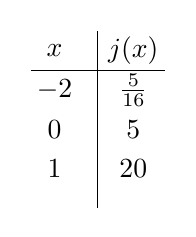
\begin{tikzpicture}
\draw(0,2)node{$x$}(1,2)node{$j(x)$};
\draw(0,1.5)node{$-2$}(1,1.5)node{$\frac{5}{16}$};
\draw(0,1)node{$0$}(1,1)node{$5$};
\draw(0,.5)node{$1$}(1,.5)node{$20$};
\draw(-.3,1.75)--(1.4,1.75);
\draw(0.55,2.25)--(0.55,0);
\end{tikzpicture}

Above are $3$ values for the function $j$.  If $j(k)=ab^{k}$ for
some constants $a$ and $b$, what is the value of $b$?



\ifsat
	\begin{enumerate}[label=\Alph*)]
		\item $\frac{1}{4}$
		\item $\frac{1}{2}$
		\item $4$%
		\item $8$
	\end{enumerate}
\else
\fi

\ifacteven
	\begin{enumerate}[label=\textbf{\Alph*.},itemsep=\fill,align=left]
		\setcounter{enumii}{5}
		\item $\frac{1}{4}$
		\item $\frac{1}{2}$
		\item $2$
		\addtocounter{enumii}{1}
		\item $4$%
		\item $8$
	\end{enumerate}
\else
\fi

\ifactodd
	\begin{enumerate}[label=\textbf{\Alph*.},itemsep=\fill,align=left]
		\item $\frac{1}{4}$
		\item $\frac{1}{2}$
		\item $2$
		\item $4$%
		\item $8$
	\end{enumerate}
\else
\fi

\ifgridin
 $4$%
		
\else
\fi

